\subsection{Pruebas del sistema}
La estrategia de validación se estructura en seis dimensiones de evidencia: pruebas unitarias, instrumentadas de interfaz, extremo a extremo, Macrobenchmark, aceptación de usuario y compatibilidad. Este enfoque garantiza la evaluación de cada componente desde perspectivas aisladas e integradas, permitiendo disociar la lógica interna de la interacción visual en Android.

Al segmentar las pruebas, se asegura la robustez de los flujos críticos y se facilita la identificación temprana de fallos en capas específicas. Asimismo, el proceso integra la percepción de los estudiantes mediante pruebas de aceptación para validar la utilidad de las funciones desarrolladas. Esta combinación de métricas técnicas y retroalimentación directa asegura el cumplimiento de los estándares de calidad y las expectativas de la comunidad universitaria:

\begin{enumerate}
  \item Pruebas unitarias automatizadas

Las pruebas unitarias se ejecutaron sobre el módulo app mediante Gradle. La suite cubre lógica de dominio, generación de horarios, filtrado de candidatos e importación de horarios compartidos.

También incluye sincronización automática, utilitarios de series, notificaciones de Simón y el estado del ViewModel. Esta cobertura permite verificar reglas críticas sin depender de un dispositivo físico. Los componentes evaluados y la naturaleza de las evidencias generadas se resumen en la Tabla \ref{tab:qa_unitarias_sistema}:

\begin{center}
\begin{minipage}{\linewidth}
\centering
\begin{tabularx}{\linewidth}{@{}p{3.4cm}>{\RaggedRight\arraybackslash}X>{\RaggedRight\arraybackslash}p{4.2cm}@{}}
\toprule
Componente & Aspecto verificado & Clases de evidencia \\
\midrule
Generador de horarios & Selección de grupos, materias obligatorias, materias opcionales, penalización por choques, docentes favoritos y colores deterministas. & Generador, filtro de candidatos y constructor de candidatos. \\
Interoperabilidad y sincronización & Importación de horarios compartidos, actualización de carreras deshabilitadas, sincronización automática y cálculo de avance académico. & Importación, sincronización y avance académico. \\
Jerarquía académica & Exclusión de materias inscritas o aprobadas y detección de conflictos al construir opciones agregables. & Jerarquía agregable y series de materias. \\
Asistente Simón & Parseo de respuestas, construcción de plantillas, planificación de recordatorios y conversión a notificaciones. & Parser, plantillas, planificador y notificaciones. \\
Presentación del generador & Carga inicial, sincronización automática, navegación a resultados y mensajes cuando no existen horarios válidos. & ViewModel del generador. \\
\bottomrule
\end{tabularx}
\captionof{table}{Cobertura de pruebas unitarias automatizadas.}\label{tab:qa_unitarias_sistema}
Fuente: Elaboración propia.
\end{minipage}
\end{center}

La validación técnica se ejecutó mediante ./gradlew :app:testDebugUnitTest, activando JUnit para procesar sistemáticamente la lógica de negocio del módulo principal. Esta tarea permite realizar verificaciones exhaustivas sobre las reglas de dominio. Así, se asegura que cada unidad de código responda con precisión a los requerimientos funcionales establecidos.

Tras la ejecución, el sistema genera automáticamente un reporte HTML en el directorio de construcción. Este recurso facilita la auditoría técnica de cada caso de prueba y permite analizar los tiempos de respuesta. Además, favorece la detección temprana de posibles regresiones en los componentes críticos de la arquitectura.

Como resultado registrado, la suite finalizó con un estado satisfactorio, completando 89 pruebas con un éxito total del 100\%. La evidencia visual de la ejecución por terminal, que confirma la integridad de los componentes evaluados, se muestra en la Figura \ref{fig:qa_unit_tests_terminal}.

\begin{figure}[H]
\centering
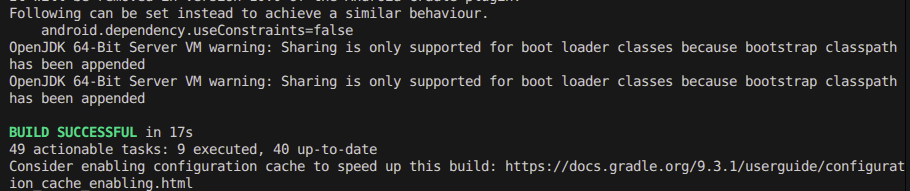
\includegraphics[width=1\linewidth]{images/pruebas/qa_unit_tests_terminal.png}
\caption[Ejecución satisfactoria de pruebas unitarias]{Ejecución satisfactoria de pruebas unitarias mediante Gradle.}\label{fig:qa_unit_tests_terminal}
Fuente: Elaboración propia.
\end{figure}

El reporte generado muestra el resumen consolidado de los casos ejecutados, fallos y duración, permitiendo verificar de forma rápida el éxito global de la suite. Como se observa en la Figura \ref{fig:qa_unit_tests_report}, la interfaz del reporte facilita la navegación entre los distintos módulos evaluados:

\begin{figure}[H]
\centering
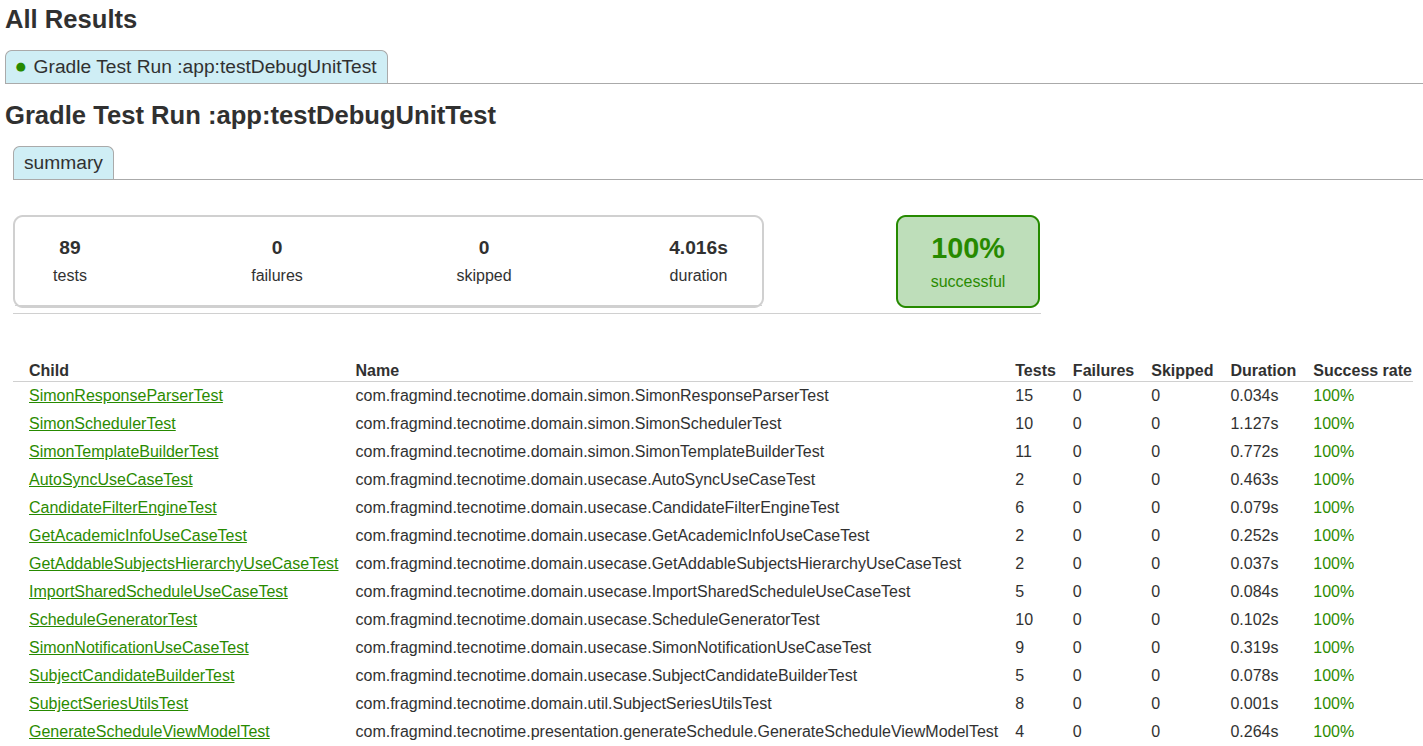
\includegraphics[width=1\linewidth]{images/pruebas/qa_unit_tests_report.png}
\caption[Reporte HTML de pruebas unitarias]{Reporte HTML de pruebas unitarias generado por Gradle.}\label{fig:qa_unit_tests_report}
Fuente: Elaboración propia.
\end{figure}

Para profundizar en el análisis técnico, los resultados detallados por cada clase de prueba, extraídos directamente de los archivos de reporte generados durante la compilación, se presentan en la Tabla \ref{tab:qa_unitarias_resultado}:

\begin{center}
\begin{minipage}{\linewidth}
\centering
\begin{tabularx}{\linewidth}{@{}>{\RaggedRight\arraybackslash}X p{1.5cm}p{1.5cm}p{1.6cm}p{1.8cm}@{}}
\toprule
Clase de prueba & Casos & Fallos & Omitidas & Duración \\
\midrule
SimonResponseParserTest & 15 & 0 & 0 & 0.029 s \\
SimonSchedulerTest & 10 & 0 & 0 & 0.807 s \\
SimonTemplateBuilderTest & 11 & 0 & 0 & 0.141 s \\
SimonNotificationUseCaseTest & 9 & 0 & 0 & 0.230 s \\
ScheduleGeneratorTest & 10 & 0 & 0 & 0.082 s \\
CandidateFilterEngineTest & 6 & 0 & 0 & 0.060 s \\
SubjectCandidateBuilderTest & 5 & 0 & 0 & 0.043 s \\
ImportSharedScheduleUseCaseTest & 5 & 0 & 0 & 0.095 s \\
AutoSyncUseCaseTest & 2 & 0 & 0 & 0.183 s \\
GetAcademicInfoUseCaseTest & 2 & 0 & 0 & 0.264 s \\
GetAddableSubjectsHierarchyUseCaseTest & 2 & 0 & 0 & 0.036 s \\
SubjectSeriesUtilsTest & 8 & 0 & 0 & 0.001 s \\
GenerateScheduleViewModelTest & 4 & 0 & 0 & 1.875 s \\
Total & 89 & 0 & 0 & 4.174 s \\
\bottomrule
\end{tabularx}
\captionof{table}{Resultados de ejecución de pruebas unitarias automatizadas.}\label{tab:qa_unitarias_resultado}
Fuente: Elaboración propia.
\end{minipage}
\end{center}

  \item Pruebas instrumentadas de interfaz

Las pruebas instrumentadas validan la interfaz en dispositivos reales, verificando la respuesta táctil y el comportamiento visual del paquete instalado. La suite utiliza Jetpack Compose Testing, ActivityScenario y Hilt para ejecutar los casos de prueba y las validaciones de contexto resumidas en el Cuadro \ref{tab:qa_ui_instrumentadas}:

\begin{center}
\begin{minipage}{\linewidth}
\centering
\begin{tabularx}{\linewidth}{@{}p{1.7cm}>{\RaggedRight\arraybackslash}X>{\RaggedRight\arraybackslash}p{3.1cm}>{\RaggedRight\arraybackslash}p{2.8cm}@{}}
\toprule
Caso & Escenario validado & Clase & Resultado \\
\midrule
UI-01 & Carga inicial de MainActivity y validación de estado de ciclo de vida iniciado o reanudado. & Actividad principal & Aprobado, 1 caso. \\
UI-02 & Apertura del menú flotante y visualización de las acciones Agregar materia, Generar horario y Agregar nota. & Componentes Compose & Aprobado. \\
UI-03 & Ejecución del botón primario Comenzar en el componente de bienvenida. & Componentes Compose & Aprobado. \\
UI-04 & Cambio de estado de un interruptor unificado de configuración. & Componentes Compose & Aprobado. \\
UI-05 & Visualización de mensaje cuando el generador no produce resultados. & Resultados del generador & Aprobado. \\
UI-06 & Visualización de horario generado y aplicación de selección completa. & Resultados del generador & Aprobado. \\
UI-07 & Validación del nombre de paquete y recursos Android disponibles. & Prueba de contexto & Aprobado, 1 caso. \\
\bottomrule
\end{tabularx}
\captionof{table}{Registro de pruebas instrumentadas de interfaz.}\label{tab:qa_ui_instrumentadas}
Fuente: Elaboración propia.
\end{minipage}
\end{center}

La ejecución de las pruebas instrumentadas se realizó mediante el comando ./gradlew :app:connectedDebugAndroidTest sobre un dispositivo físico real. Esta instrucción activa el despliegue del paquete de pruebas y sincroniza el ejecutor con el hardware para garantizar un entorno de validación fiel a la experiencia del usuario final.

Dicho proceso automatiza la interacción con los componentes desarrollados en Jetpack Compose, simulando gestos precisos para validar la respuesta táctil y la navegación entre pantallas. Esta verificación asegura la estabilidad de los flujos visuales bajo condiciones de uso normal y la correcta gestión de recursos en el dispositivo.

La suite finalizó de forma satisfactoria con 7 casos completados y un éxito total del 100\% en el entorno de prueba. La evidencia visual de la ejecución por terminal, registrada en la Figura \ref{fig:qa_ui_tests_terminal}, confirma que los componentes de la interfaz responden correctamente a las interacciones automatizadas sin reportar fallos de renderizado o estados inconsistentes.

\begin{figure}[H]
\centering
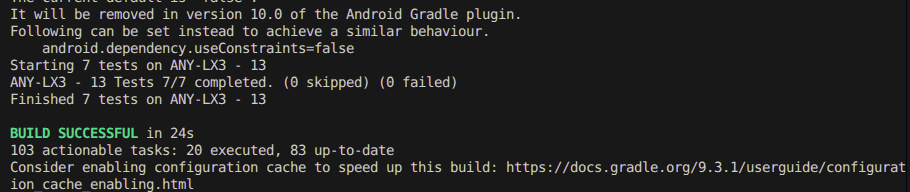
\includegraphics[width=1\linewidth]{images/pruebas/qa_ui_tests_terminal.png}
\caption[Ejecución de pruebas instrumentadas de interfaz]{Ejecución de pruebas instrumentadas de interfaz mediante Gradle.}\label{fig:qa_ui_tests_terminal}
Fuente: Elaboración propia.
\end{figure}

Para un análisis más detallado, el reporte consolidado permite revisar los casos ejecutados, su estado final y el tiempo de ejecución específico por cada clase de prueba. Los resultados granulares de esta suite de validación visual se detallan en la Figura \ref{fig:qa_ui_tests_report}, sirviendo como respaldo técnico de la estabilidad de la UI ante diversos escenarios de uso.

\begin{figure}[H]
\centering
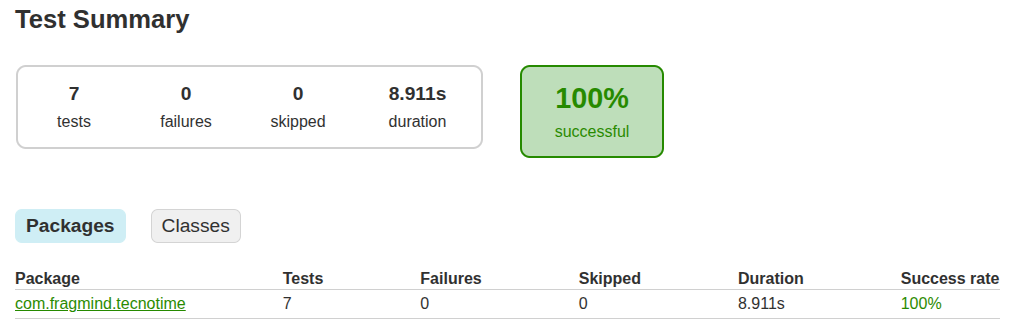
\includegraphics[width=1\linewidth]{images/pruebas/qa_ui_tests_report.png}
\caption[Reporte HTML de pruebas instrumentadas]{Reporte HTML de pruebas instrumentadas de interfaz generado por Gradle.}\label{fig:qa_ui_tests_report}
Fuente: Elaboración propia.
\end{figure}

  \item Pruebas de extremo a extremo

Las pruebas de extremo a extremo (E2E) se enfocan en la validación de flujos críticos que atraviesan múltiples capas de la arquitectura del sistema. A diferencia de las pruebas unitarias, estas verifican la integración real entre la interfaz de usuario, la lógica de dominio y la capa de persistencia local en un entorno de ejecución completo.

La ejecución de estas pruebas asegura que los componentes desacoplados funcionen armoniosamente en un entorno integrado, minimizando el riesgo de errores de comunicación entre módulos. La trazabilidad completa entre los flujos críticos evaluados y las evidencias de validación correspondientes se presenta en la Tabla \ref{tab:qa_e2e_resultados}:

\begin{center}
\begin{minipage}{\linewidth}
\centering
\begin{tabularx}{\linewidth}{@{}p{1.8cm}>{\RaggedRight\arraybackslash}X>{\RaggedRight\arraybackslash}X>{\RaggedRight\arraybackslash}p{3.4cm}@{}}
\toprule
Código & Flujo & Procedimiento & Evidencia \\
\midrule
E2E-01 & Inicio y pantalla principal & Instalar la variante debug, iniciar la aplicación y verificar que la actividad principal queda iniciada o reanudada. & Prueba de actividad. \\
E2E-02 & Menú de acciones & Abrir Más opciones y comprobar las acciones principales. & Prueba de menú. \\
E2E-03 & Generación automática & Abrir Generar horario, ejecutar Go y esperar resultados o mensaje controlado. & Macrobenchmark. \\
E2E-04 & Aplicación de horario generado & Mostrar una propuesta generada y aplicar la selección completa. & Prueba de resultados. \\
E2E-05 & Exportación y recordatorios & Verificar exportación, evento académico y notificación programada con ejecución manual supervisada. & Capturas de aplicación. \\
\bottomrule
\end{tabularx}
\captionof{table}{Flujos de extremo a extremo y evidencia asociada.}\label{tab:qa_e2e_resultados}
Fuente: Elaboración propia.
\end{minipage}
\end{center}

En la validación automatizada de extremo a extremo (E2E), se priorizó el flujo de generación de horarios por ser la funcionalidad central. Mediante UI Automator y ComposeTestRule, se verificó que el disparador de generación, gestionado por el ViewModel, sea plenamente accesible. Esta integración asegura una navegación fluida y sincronización mediante StateFlow.

El motor ScheduleGenerator y el componente CandidateFilterEngine respondieron de manera previsible ante restricciones combinatorias. Se validó el procesamiento de grafos de materias para emitir propuestas viables o mensajes controlados en situaciones de conflicto. Esta robustez, validada con Hilt, garantiza una retroalimentación técnica clara al usuario.

  \item Pruebas de carga y rendimiento

Las pruebas de carga se plantearon bajo un enfoque adaptado al modelo offline-first y al procesamiento local intensivo. En este paradigma de computación en el borde (Edge Computing), la carga no se define por la cantidad de usuarios concurrentes en un servidor central, sino por la capacidad de respuesta y eficiencia del hardware del cliente ante la ejecución de algoritmos complejos de optimización de horarios.

Se evaluó de forma exhaustiva el estrés de recursos críticos como CPU, memoria RAM y almacenamiento interno. Mediante operaciones intensivas repetidas, se identificó el límite de estabilidad del sistema. Esto asegura que la gestión de memoria evite cierres inesperados durante procesos de alta demanda computacional en el dispositivo móvil.

Para obtener mediciones precisas, se incorporó un módulo de :macrobenchmark en la estructura del proyecto. La suite utiliza AndroidX Macrobenchmark con UI Automator y una variante de compilación no depurable. Los escenarios de rendimiento automatizados que componen esta evaluación se detallan exhaustivamente en la Tabla \ref{tab:qa_macrobenchmark_escenarios}:

\begin{center}
\begin{minipage}{\linewidth}
\centering
\begin{tabularx}{\linewidth}{@{}p{2cm}>{\RaggedRight\arraybackslash}X>{\RaggedRight\arraybackslash}p{2.6cm}>{\RaggedRight\arraybackslash}X@{}}
\toprule
Escenario & Procedimiento & Iteraciones & Métricas \\
\midrule
MB-01 & Inicio en frío de la aplicación. & 10 & timeToInitialDisplayMs. \\
MB-02 & Navegación y desplazamiento en la pantalla principal. & 5 & frameDurationCpuMs, frameOverrunMs, cantidad de cuadros. \\
MB-03 & Flujo de generación automática de horarios desde el menú principal. & 5 & GenerarHorarioFlowCount y GenerarHorarioFlowSumMs. \\
\bottomrule
\end{tabularx}
\captionof{table}{Escenarios automatizados de rendimiento con Macrobenchmark.}\label{tab:qa_macrobenchmark_escenarios}
Fuente: Elaboración propia.
\end{minipage}
\end{center}

La evaluación del rendimiento se ejecutó mediante el comando ./gradlew :macrobenchmark:connectedBenchmarkAndroidTest en un entorno de pruebas optimizado. Esta instrucción activa la suite de Macrobenchmark, que realiza múltiples iteraciones sobre los flujos críticos para capturar métricas estables de latencia y suavidad de la interfaz. De este modo, se asegura que las mediciones obtenidas sean representativas y no se vean alteradas por ruidos térmicos o procesos externos del dispositivo móvil.

El reporte HTML generado desglosa percentiles y trazas de CPU para identificar cuellos de botella en Jetpack Compose. Esta documentación técnica, almacenada junto a trazas de Perfetto para auditoría, valida la estabilidad del sistema en el Cuadro \ref{tab:qa_macrobenchmark_resultados}:

\begin{center}
\begin{minipage}{\linewidth}
\centering
\begin{tabularx}{\linewidth}{@{}p{2.4cm}>{\RaggedRight\arraybackslash}X>{\RaggedRight\arraybackslash}p{3.2cm}>{\RaggedRight\arraybackslash}p{2.2cm}@{}}
\toprule
Escenario & Métrica principal & Resultado & Estado \\
\midrule
MB-01 & Tiempo hasta primera visualización. & Mediana: 592.20 ms; mínimo: 518.63 ms; máximo: 1089.26 ms. & Aprobado. \\
MB-02 & Duración de cuadros en CPU. & P50: 4.85 ms; P95: 10.72 ms; P99: 13.51 ms. & Aprobado. \\
MB-02 & Sobrecosto de cuadro. & P95: -2.82 ms, sin excedente crítico en la medición registrada. & Aprobado. \\
MB-03 & Traza GenerarHorarioFlow. & Mediana: 155.28 ms; ejecuciones: 148.60, 155.28, 153.86, 157.33 y 157.53 ms. & Aprobado. \\
MB-03 & Conteo de traza. & Mediana: 1; una generación real por iteración. & Aprobado. \\
\bottomrule
\end{tabularx}
\captionof{table}{Resultados de rendimiento obtenidos con Macrobenchmark.}\label{tab:qa_macrobenchmark_resultados}
Fuente: Elaboración propia.
\end{minipage}
\end{center}

La Figura \ref{fig:qa_macrobenchmark_report} presenta la evidencia visual del reporte de rendimiento, detallando trazas de ejecución y percentiles de latencia. Esta documentación confirma la fluidez de la interfaz y la estabilidad del sistema bajo carga de trabajo intensiva.

\begin{figure}[H]
\centering
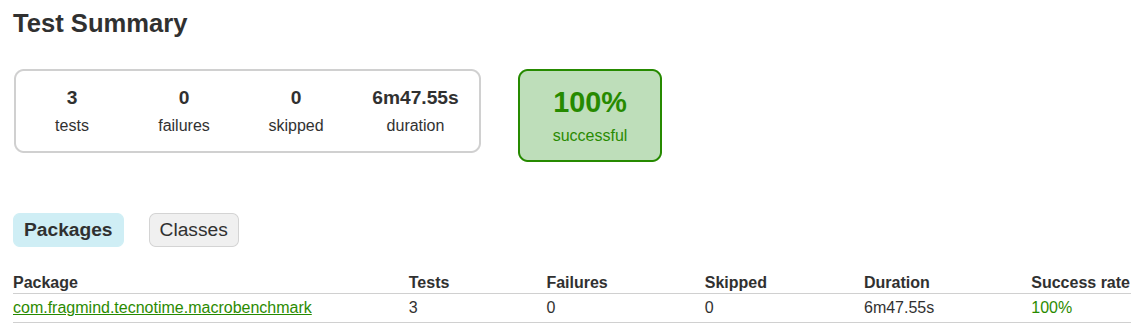
\includegraphics[width=1\linewidth]{images/pruebas/qa_macrobenchmark_report.png}
\caption[Reporte de rendimiento Macrobenchmark]{Reporte de rendimiento generado por AndroidX Macrobenchmark.}\label{fig:qa_macrobenchmark_report}
Fuente: Elaboración propia.
\end{figure}

La ejecución constituye evidencia técnica válida en el dispositivo HONOR/Huawei evaluado. Se garantizó la estabilidad mediante un entorno sin diálogos del sistema y la configuración dropShaders.enable=false, asegurando la compatibilidad con el receptor de ProfileInstaller.

  \item Pruebas de aceptación de usuario

Las pruebas de aceptación (UAT) validan la autonomía del estudiante mediante un piloto de 15 alumnos de Ingeniería Química e Informática (FCyT), representativos del estudio de campo previo. Los escenarios ejecutados se resumen en el Cuadro \ref{tab:qa_uat_escenarios}:

\begin{center}
\begin{minipage}{\linewidth}
\centering
\begin{tabularx}{\linewidth}{@{}p{1.8cm}>{\RaggedRight\arraybackslash}X>{\RaggedRight\arraybackslash}X>{\RaggedRight\arraybackslash}p{3.2cm}@{}}
\toprule
Código & Escenario & Procedimiento & Evidencia \\
\midrule
UAT-01 & Configuración inicial & Registrar datos básicos y completar el flujo de bienvenida. & Captura y tiempo de ejecución. \\
UAT-02 & Selección académica & Seleccionar carrera, nivel, materia y grupo. & Capturas del flujo. \\
UAT-03 & Visualización del horario & Verificar que las materias agregadas aparezcan en la vista semanal. & Captura del horario. \\
UAT-04 & Generación automática & Generar alternativas de horario y seleccionar una opción válida. & Captura de resultados. \\
UAT-05 & Eventos y recordatorios & Crear un evento académico y activar recordatorios. & Captura de formulario y notificación. \\
UAT-06 & Exportación o compartición & Generar un archivo o contenido compartible del horario. & Captura del archivo generado. \\
UAT-07 & Asistente Simón & Activar notificaciones inteligentes y verificar un mensaje generado. & Captura de notificación. \\
\bottomrule
\end{tabularx}
\captionof{table}{Escenarios definidos para las pruebas de aceptación de usuario.}\label{tab:qa_uat_escenarios}
Fuente: Elaboración propia.
\end{minipage}
\end{center}

Para medir la mejora de experiencia frente a herramientas existentes se definieron indicadores comparables. Las métricas de desempeño y satisfacción proyectadas para esta fase se resumen en la Tabla \ref{tab:qa_uat_metricas}:

\begin{center}
\begin{minipage}{\linewidth}
\centering
\begin{tabularx}{\linewidth}{@{}p{4.2cm}>{\RaggedRight\arraybackslash}X>{\RaggedRight\arraybackslash}p{3cm}@{}}
\toprule
Indicador & Cálculo & Resultado \\
\midrule
Tasa de finalización & Tareas completadas / tareas asignadas $\times$ 100. & 100\% (15/15). \\
Tiempo (Bienvenida) & Tiempo promedio en flujo inicial. & 35 segundos. \\
Tiempo (Generación) & Tiempo promedio en motor de horarios. & 22 segundos. \\
Errores críticos & Fallos que impiden completar la tarea. & 0\%. \\
Satisfacción general & Promedio de respuestas Likert de 1 a 5. & 4.6 / 5.0. \\
Facilidad de uso & Promedio de respuestas sobre navegación. & 4.4 / 5.0. \\
\bottomrule
\end{tabularx}
\captionof{table}{Resultados de aceptación y métricas de experiencia de usuario.}\label{tab:qa_uat_metricas}
Fuente: Elaboración propia.
\end{minipage}
\end{center}

Los resultados del piloto confirman una alta tasa de aceptación, con el total de los participantes completando los flujos críticos. Se observó una leve curva de aprendizaje en dos estudiantes respecto al formulario de parámetros del generador, quienes requirieron un tiempo adicional para comprender las restricciones de búsqueda antes de obtener sus resultados satisfactoriamente.

La eficiencia del sistema destaca en la generación de horarios, logrando tiempos de respuesta de entre 10 y 30 segundos una vez configuradas las materias. Con un promedio de satisfacción de 4.6 sobre 5.0, los datos respaldan la viabilidad técnica y funcional de la aplicación en el contexto académico evaluado, cumpliendo con las expectativas de facilidad de uso de la comunidad universitaria.

  \item Pruebas de compatibilidad

Las pruebas de compatibilidad verifican que la aplicación se instale, inicie y mantenga sus flujos principales en el entorno de ejecución objetivo. Esta validación es crítica dado el ecosistema fragmentado de Android, por lo que se priorizó el uso de dispositivos físicos que representen la gama media utilizada por los estudiantes de la facultad.

La selección se centra en un dispositivo con capacidades de hardware estándar y una versión de sistema operativo representativa del mercado actual. El entorno físico definido para documentar la compatibilidad del sistema se especifica en la Tabla \ref{tab:qa_compat_entornos}:

\begin{center}
\begin{minipage}{\linewidth}
\centering
\begin{tabularx}{\linewidth}{@{}p{1.8cm}>{\RaggedRight\arraybackslash}X>{\RaggedRight\arraybackslash}p{2.8cm}>{\RaggedRight\arraybackslash}p{2.6cm}>{\RaggedRight\arraybackslash}p{2.6cm}@{}}
\toprule
Código & Entorno & Versión & Resolución & Hardware \\
\midrule
COMP-01 & Dispositivo físico validado & Android 13, API 33 & 1080x2388, 480 dpi & HONOR ANY-LX3, 8 núcleos, 7.9 GB RAM \\
\bottomrule
\end{tabularx}
\captionof{table}{Entorno físico definido para pruebas de compatibilidad.}\label{tab:qa_compat_entornos}
Fuente: Elaboración propia.
\end{minipage}
\end{center}

La selección de este hardware específico permitió validar la gestión de recursos bajo una densidad de píxeles y potencia de procesamiento representativa de la gama media. Se puso especial énfasis en la estabilidad del motor de renderizado y la persistencia de datos locales, confirmando que la arquitectura desacoplada del sistema responde con eficiencia ante las especificaciones técnicas del dispositivo físico evaluado.

En este entorno se comprobó la instalación del paquete de aplicación, el inicio exitoso y la ejecución de los flujos críticos de usuario sin degradación del rendimiento. El registro consolidado de los resultados de compatibilidad obtenidos en el dispositivo de prueba se presenta en el Cuadro \ref{tab:qa_compat_resultados}:

\begin{center}
\begin{minipage}{\linewidth}
\centering
\begin{tabularx}{\linewidth}{@{}p{1.8cm}>{\RaggedRight\arraybackslash}X>{\RaggedRight\arraybackslash}p{3.2cm}>{\RaggedRight\arraybackslash}p{2.7cm}@{}}
\toprule
Código & Verificación & Evidencia & Estado \\
\midrule
COMP-01 & Instalación, inicio, pruebas instrumentadas y Macrobenchmark en dispositivo físico. & Reportes Gradle, Android Test, Macrobenchmark y trazas Perfetto. & Validado. \\
\bottomrule
\end{tabularx}
\captionof{table}{Registro de resultados de compatibilidad.}\label{tab:qa_compat_resultados}
Fuente: Elaboración propia.
\end{minipage}
\end{center}

Adicionalmente, la compatibilidad extendida con el resto del ecosistema Android se gestiona y verifica mediante la consola de Google Play, la cual proporciona un catálogo de miles de modelos certificados que cumplen con los requisitos mínimos del sistema. Esta estrategia asegura que la aplicación sea funcional en una amplia variedad de terminales sin requerir pruebas manuales exhaustivas en cada modelo individual.
\end{enumerate}
